\documentclass{standalone}
\usepackage{tikz}
\usepackage{newtxmath}
\usetikzlibrary{calc}

\begin{document}

\definecolor{darkred}{RGB}{200,0,0}
\colorlet{lightred}{red!80!black}
\definecolor{newgreen}{RGB}{33,172,47}
\definecolor{newblue}{RGB}{43,174,222}
\colorlet{darkgreen}{green!50!black}
\colorlet{lightgreen}{green!80!black}

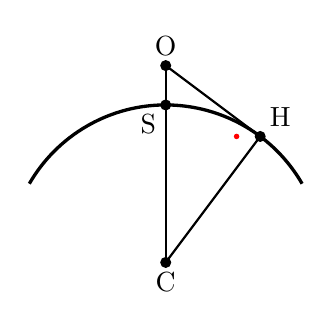
\begin{tikzpicture}

\coordinate (O) at (0, 0);

\fill[black] (O) circle (2pt) node[below]{C};
\draw[very thick] (O) ++(30:2) arc (30:150:2);

\fill[black] (0,2) circle (2pt) node[below left]{S};
\draw[thick] (O) -- (0,2.5);

\fill[black] (0,2.5) circle (2pt) node[above]{O};

\fill[black] (1.2,1.6) circle (2pt) node[above right]{H};
\draw[thick] (O) -- (1.2,1.6);
\draw[thick] (0,2.5) -- (1.2,1.6);
\fill[red] (0.9,1.6) circle (1pt);

\end{tikzpicture}


\end{document}